% !Mode:: "TeX:UTF-8"

\chapter{BFGS}

问题: 求函数$f(x)$的最小值,即:
\begin{displaymath}
x^*=argmin(f(x))
\end{displaymath} 

\section{牛顿法}
假设我们可以构造一个序列$f(x_0), f(x_1), f(x_2), ..., f(x_n), ...$,使得$f(x_i)>f(x_{i+1}$,并且当$i \rightarrow \infty$时,$f(x_i) \rightarrow min(f(x))$.

假设$f(x)$是二次可导的,则可以用该函数在$x$处的二阶泰勒展开作为该函数的近似:
\begin{displaymath}
f(x+\Delta x) \approx \frac{f(x)}{0!} + \frac{\Delta x^T\bigtriangledown f(x)}{1!}+ \frac{\Delta x^T\bigtriangledown^2f(x)\Delta x}{2!} 
\end{displaymath}
其中, $\bigtriangledown f(x)$和$\bigtriangledown^2f(x)$分别是$f(x)$在点$x$处的梯度和Hessian矩阵。我们令$x_{n+1}=x_n+\Delta x$,并将上公式改写为:
\begin{displaymath}
h_n(\Delta x)=f(x_n)+\Delta x^T\mathbf{g}_n +\frac{1}{2}\Delta x^T \mathbf{H}_n\Delta x
\end{displaymath}
其中, $\mathbf{g}_n$和$\mathbf{H}_n$分别是$f(x)$在点$x_n$处的梯度和Hessian矩阵。

为得到原始函数$f(x)$的最小值,我们现在有其在点$x_n$处的近似,我们可以将点$x_n$移动到点$x_n + \Delta x$处获得一个更小值,那么如何选择$\Delta x$。基于近似函数$h_n(\Delta x)$,我们选择使得该近似函数最小的$\Delta x$,由于该近似函数为凸函数(假设$\mathbf{H}_n$为正定矩阵),全局最小值处导数为0,故而:
\begin{displaymath}
\frac{\partial h_n(\Delta x)}{\partial \Delta x} = \mathbf{g}_n + \mathbf{H}_n \Delta x = 0
\end{displaymath}
从而得到一个比较好的基于当前点$x_n$的移动方向$\Delta x$:
\begin{displaymath}
\Delta x = -\mathbf{H}_n^{-1}\mathbf{g}_n
\end{displaymath}

从而我们有牛顿优化算法如下:

\begin{minipage}{0.8\textwidth}\centering
\begin{algorithm}[H]
\textbf{NewtonRaphson}($f$,$x_0$):\\
\For{n=0,1,...(until converged)}{
Compute $\mathbf{g}_n$ and $\mathbf{H}_n^{-1}$ for $x_n$\\
$d=\mathbf{H}_n^{-1}\mathbf{g}_n$\\
$x_{n+1} \leftarrow x_n - d$\\
}
\end{algorithm}
\end{minipage}

\section{阻尼牛顿法}

由于函数$h_n(\Delta x)$仅仅为原始函数的近似,故而该函数的最低点并不一定是原始函数的最低点,如果一次更新到该近似函数的极值点可能会导致$f(x_{n+1}) > f(x_n)$的情况发生。一个比较合理的选择是向方向$d$移动一段距离,即引入步长$\alpha$。步长$\alpha$的计算可以任意的线性搜索算法来得到。

\begin{minipage}{0.8\textwidth}\centering
\begin{algorithm}[H]
\textbf{NewtonRaphson}($f$,$x_0$):\\
\For{n=0,1,...(until converged)}{
Compute $\mathbf{g}_n$ and $\mathbf{H}_n^{-1}$ for $x_n$\\
$d=\mathbf{H}_n^{-1}\mathbf{g}_n$\\
$\alpha = \min \limits_{\alpha \geqq 0} f(x_n-\alpha d)$\\
$x_{n+1} \leftarrow x_n - \alpha d$\\
}
\end{algorithm}
\end{minipage}
 
牛顿法和阻尼牛顿法都需要对Hessian矩阵$\mathbf{H}$进行计算(函数参数为$N$,计算量为$N^2$)。当函数参数比较多时,每次更新的计算量比较大。如何计算一个近似的矩阵来替代Hessian矩阵成为加速牛顿法的主要思路,该一系列方法成为拟牛顿法。

\section{拟牛顿法}
拟牛顿法的基本思想是使用一个近似矩阵来模拟Hessian矩阵。那么什么样的矩阵才适合作为Hessian矩阵的近似呢?基于前面近似函数:
\begin{displaymath}
h_n(\Delta x)=f(x_n)+\Delta x^T\mathbf{g}_n +\frac{1}{2}\Delta x^T \mathbf{H}_n\Delta x
\end{displaymath}
一个好的近似函数应该满足在点$x_{n+1}$和$x_n$处的一阶导数同原始函数一致,即:
\begin{displaymath}
\begin{split}
\Delta h_n(x_n) &= \mathbf{g}_n\\
\Delta h_n(x_{n+1}) &= \mathbf{g}_{n+1}
\end{split}
\end{displaymath}
从而有:
\begin{displaymath}
\Delta h_n(x_{n+1}) -\Delta h_n(x_n) = \mathbf{g}_{n+1} - \mathbf{g}_n
\end{displaymath}
根据中值定理在点$x_n$和$x_{n+1}$之间存在某点$x_n^{'}$该处的Hessian矩阵$B_{n+1}$满足:
\begin{displaymath}
B_{n+1}(x_{n+1} - x_n) = \Delta h_n(x_{n+1}) -\Delta h_n(x_{n})  = \mathbf{g}_{n+1} - \mathbf{g}_n
\end{displaymath}

% \begin{figure}[htbp]
% \centering
% 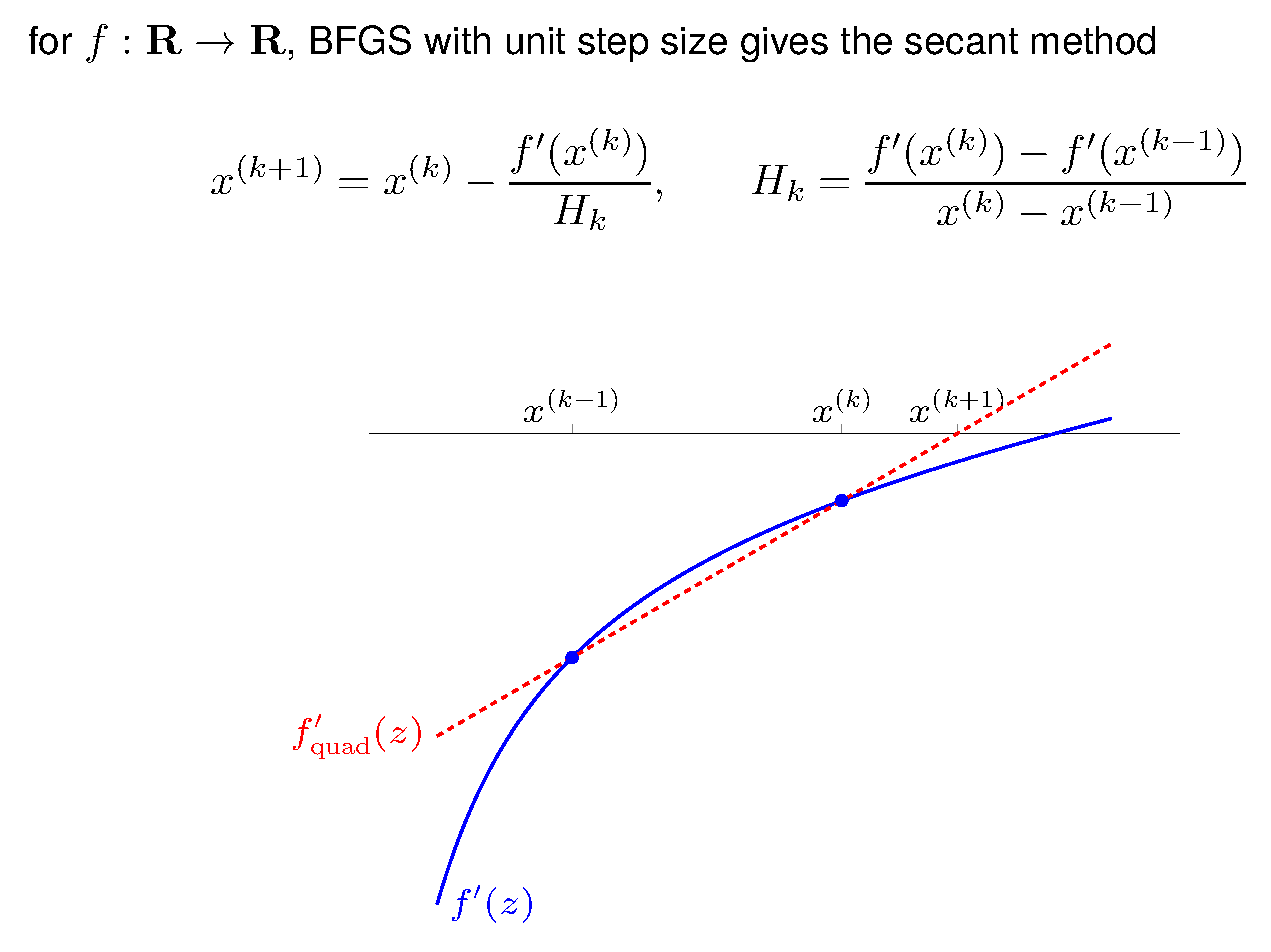
\includegraphics[width = 0.8\textwidth]{SecantCondition}
% \end{figure}

我们令$\mathbf{s}_n=x_{n+1}-x_{n}$,$\mathbf{y}_n=\mathbf{g}_{n+1} - \mathbf{g}_n$,$D_n = B_n^{-1}$则有:
\begin{displaymath}
\begin{split}
B_{n+1}\mathbf{s}_n = \mathbf{y}_n\\
\mathbf{s}_n = D_{n+1} \mathbf{y}_n
\end{split}
\end{displaymath}
该约束条件称为Secant条件。Secant条件可以保证选取的近似Hessian矩阵使得近似函数在点$x_{n-1}$和$x_n$处的一阶导数同原始函数一致。


\section{DFP算法}
DFP算法是由Davidon, Fletcher, Powell三人提出的拟牛顿法。DFP算法的基本思路是从一个对称矩阵$D_0$开始,采用迭代的方式$D_{n+1}=D_n+\Delta D_n, n=0,1,2,...$来获得一个Hessian逆矩阵的近似矩阵。那么如何计算$\Delta D_n$。我们知道如果$D_n$是对称矩阵,那么只要$\Delta D_n$为对称矩阵,则得到的$D_{n+1}$也为对称矩阵。不失一般性的,我们假设$\Delta D_n$的形式为$\Delta D_n = \alpha\mathbf{uu}^T + \beta \mathbf{vv}^T$,其中$\alpha$和$\beta$为待定参数,$\mathbf{u}$和$\mathbf{v}$为待定向量。

根据Secant条件我们有:
\begin{displaymath}
\begin{split}
\mathbf{s}_n &= D_{n+1} \mathbf{y}_n\\
 &= (D_n + \Delta D) \mathbf{y}_n\\
 &= (D_n + \alpha\mathbf{uu}^T + \beta \mathbf{vv}^T) \mathbf{y}_n\\
 &= (D_n + \alpha\mathbf{uu}^T + \beta \mathbf{vv}^T) \mathbf{y}_n\\
\mathbf{s}_n &= D_n \mathbf{y}_n + \alpha\mathbf{uu}^T \mathbf{y}_n + \beta \mathbf{vv}^T \mathbf{y}_n\\
&= D_n \mathbf{y}_n + (\alpha\mathbf{u}^T \mathbf{y}_n)\mathbf{u} + (\beta \mathbf{v}^T \mathbf{y}_n)\mathbf{v}
\end{split}
\end{displaymath}
令$\alpha=\frac{1}{\mathbf{u}^T \mathbf{y}_n}$,$\beta = \frac{-1}{\mathbf{v}^T \mathbf{y}_n}$,则有:
\begin{displaymath}
\begin{split}
\mathbf{s}_n = D_n \mathbf{y}_n + \mathbf{u} -  \mathbf{v}\\
\mathbf{u} -  \mathbf{v} =\mathbf{s}_n - D_n \mathbf{y}_n 
\end{split}
\end{displaymath}

为满足secant条件,我们令$\mathbf{u}= \mathbf{s}_n$, $\mathbf{v} = D_n\mathbf{y}_n$,从而:
\begin{displaymath}
\begin{split}
\alpha &=\frac{1}{\mathbf{u}^T \mathbf{y}_n} =\frac{1}{\mathbf{s}_n^T\mathbf{y}_n}\\
\beta &= \frac{-1}{\mathbf{v}^T \mathbf{y}_n} = \frac{-1}{(D_n\mathbf{y})^T \mathbf{y}_n} = \frac{-1}{\mathbf{y}^T D_n \mathbf{y}_n}\\
\end{split}
\end{displaymath}
故而有:
\begin{displaymath}
\Delta D_n = \alpha\mathbf{uu}^T + \beta \mathbf{vv}^T
=\frac{\mathbf{uu}^T}{\mathbf{s}_n^T\mathbf{y}_n} + \frac{-\mathbf{vv}^T}{\mathbf{y}_n^T D_n \mathbf{y}_n}
=\frac{\mathbf{s}_n\mathbf{s}_n^T}{\mathbf{s}_n^T\mathbf{y}_n} - \frac{D_n\mathbf{y}_n\mathbf{y}_n^TD_n}{\mathbf{y}_n^T D_n \mathbf{y}_n}
\end{displaymath}

DFP算法具体如下:

\begin{minipage}{0.8\textwidth}\centering
\begin{algorithm}[H]
\textbf{DFP}($f$,$\epsilon$, $x_0$):\\
$D_0 = I$\\
\For{n=0,1,...(until $\lVert \mathbf{g}_n \rVert \leq \epsilon$)}{
$d_n=D_n\mathbf{g}_n$\\
$\alpha = \min \limits_{\alpha \geqq 0} f(x_n- \alpha d_n)$\\
$\mathbf{s}_n = \alpha d_n$, $x_{n+1} = x_n + \mathbf{s}_n$, $\mathbf{y}_n = \mathbf{g}_{n+1}-\mathbf{g}_n$ \\
$D_{n+1}=D_n + \frac{\mathbf{s}_n\mathbf{s}_n^T}{\mathbf{s}_n^T\mathbf{y}_n} - \frac{D_n\mathbf{y}_n\mathbf{y}_n^TD_n}{\mathbf{y}^T D_n \mathbf{y}_n}$
}
\end{algorithm}
\end{minipage}

另一个证明的思路是:
\begin{displaymath}
\begin{split}
\min & _{D_{n+1}}{\lVert D_{n+1}-D_n \rVert ^2}\\
s.t.~~~~ &s_n = D_{n+1}\mathbf{y}_n\\
&D_{n+1}~~ is~ symmetric
\end{split}
\end{displaymath}
%  条件 $D_{n+1}~~ is ~ symmetric$能够改写为 $D_{n+1} = D_n + \Delta D_n$,其中$\Delta D_n =\mathbf{uu}^T + \mathbf{vv}^T$。则优化问题变为:
% \begin{displaymath}
% \begin{split}
% \min & \limits_{\mathbf{u,v}}{\lVert \mathbf{uu}^T + \mathbf{vv}^T \rVert ^2}\\
% s.t.~~~~ &s_n = (D_n + \mathbf{uu}^T + \mathbf{vv}^T)\mathbf{y}_n\\
% &D_0=I
% \end{split}
% \end{displaymath}
% 证不下去了.....

\section{BFGS算法}

BFGS算法是由Broden, Fletcher, Goldfarb, Shanno四人提出的。同DFP算法类似,BFGS算法同样从一个对称矩阵$B_0$开始,采用迭代的方式生成近似矩阵$B_{n+1}=B_n+\Delta B_n, n=0,1,2,...$。需要指出的是DFP方法获取的是Hessian逆矩阵的近似矩阵,而BFGS方法则是获取Hessian矩阵的近似矩阵。同DFP的证明一样,我们另$\Delta B_n = \alpha \mathbf{uu}^T + \beta \mathbf{vv}^T$,其中$\alpha$和$\beta$为待定参数,$\mathbf{u}$和$\mathbf{v}$为待定向量。
\begin{figure}[htbp]
\centering
\includegraphics[width = 0.8\textwidth]{Broyden-Fletcher-Goldfarb-Shanno}
\end{figure}

根据Secant条件我们有:
\begin{displaymath}
\begin{split}
\mathbf{y}_n &= B_{n+1} \mathbf{s}_n\\
 &= (B_n + \Delta B) \mathbf{s}_n\\
 &= (B_n + \alpha\mathbf{uu}^T + \beta \mathbf{vv}^T) \mathbf{s}_n\\
 &= (B_n + \alpha\mathbf{uu}^T + \beta \mathbf{vv}^T) \mathbf{s}_n\\
\mathbf{y}_n &= B_n \mathbf{s}_n + \alpha\mathbf{uu}^T \mathbf{s}_n + \beta \mathbf{vv}^T \mathbf{s}_n\\
&= B_n \mathbf{s}_n + (\alpha\mathbf{u}^T \mathbf{s}_n)\mathbf{u} + (\beta \mathbf{v}^T \mathbf{s}_n)\mathbf{v}
\end{split}
\end{displaymath}
令$\alpha=\frac{1}{\mathbf{u}^T \mathbf{s}_n}$,$\beta = \frac{-1}{\mathbf{v}^T \mathbf{s}_n}$,则有:
\begin{displaymath}
\begin{split}
\mathbf{y}_n = B_n \mathbf{s}_n + \mathbf{u} -  \mathbf{v}\\
\mathbf{u} -  \mathbf{v} =\mathbf{y}_n - B_n \mathbf{s}_n 
\end{split}
\end{displaymath}

为满足secant条件,我们令$\mathbf{u}= \mathbf{y}_n$, $\mathbf{v} = B_n\mathbf{s}_n$,从而:
\begin{displaymath}
\begin{split}
\alpha &=\frac{1}{\mathbf{u}^T \mathbf{s}_n} =\frac{1}{\mathbf{y}_n^T\mathbf{s}_n}\\
\beta &= \frac{-1}{\mathbf{v}^T \mathbf{s}_n} = \frac{-1}{(B_n\mathbf{s}_n)^T \mathbf{s}_n} = \frac{-1}{\mathbf{s}_n^T B_n \mathbf{s}_n}\\
\end{split}
\end{displaymath}
故而有:
\begin{displaymath}
\Delta B_n = \alpha\mathbf{uu}^T + \beta \mathbf{vv}^T
=\frac{\mathbf{uu}^T}{\mathbf{y}_n^T\mathbf{s}_n} + \frac{-\mathbf{vv}^T}{\mathbf{s}_n^T B_n \mathbf{s}_n}
=\frac{\mathbf{y}_n\mathbf{y}_n^T}{\mathbf{y}_n^T\mathbf{s}_n} - \frac{B_n\mathbf{s}_n\mathbf{s}_n^TB_n}{\mathbf{s}^T B_n \mathbf{s}_n}
\end{displaymath}

BFGS算法具体如下:

\begin{minipage}{0.8\textwidth}\centering
\begin{algorithm}[H]
\textbf{BFGS}($f$,$\epsilon$, $x_0$):\\
$B_0 = I$\\
\For{n=0,1,...(until $\lVert \mathbf{g}_n \rVert \leq \epsilon$)}{
$d_n=B_n^{-1}\mathbf{g}_n$\\
$\alpha = \min \limits_{\alpha \geqq 0} f(x_n- \alpha d_n)$\\
$\mathbf{s}_n = \alpha d_n$, $x_{n+1} = x_n + \mathbf{s}_n$, $\mathbf{y}_n = \mathbf{g}_{n+1}-\mathbf{g}_n$ \\
$B_{n+1}=B_n + \frac{\mathbf{y}_n\mathbf{y}_n^T}{\mathbf{y}_n^T\mathbf{s}_n} - \frac{B_n\mathbf{s}_n\mathbf{s}_n^TB_n}{\mathbf{s}^T B_n \mathbf{s}_n}$
}
\end{algorithm}
\end{minipage}

另一个证明的思路是:
\begin{displaymath}
\begin{split}
\min & _{B_{n+1}}{\lVert B_{n+1}-B_n \rVert ^2}\\
s.t.~~~~ &y_n = B_{n+1}\mathbf{s}_n\\
&B_{n+1}~~ is~ symmetric
\end{split}
\end{displaymath}

我们看到,在BFGS算法当中我们需要计算矩阵$B_n$的逆,常用的方法是利用Sherman-Morrison公式来直接使用$B_n^{-1}$来直接计算$B_{n+1}^{-1}$:
\begin{displaymath}
\begin{split}
B_{n+1}^{-1} = \left( I- \frac{\mathbf{s}_n\mathbf{y}_n^T}{\mathbf{y}_n^T\mathbf{s}_n} \right) B_n^{-1} \left( I- \frac{\mathbf{y}_n\mathbf{s}_n^T}{\mathbf{y}_n^T\mathbf{s}_n} \right) +\frac{\mathbf{s}_n\mathbf{s}_n^T}{\mathbf{y}_n^T\mathbf{s}_n}
\end{split}
\end{displaymath}
我们令$B^{-1}=D$,则公式为
\begin{displaymath}
\begin{split}
D_{n+1} = \left( I- \frac{\mathbf{s}_n\mathbf{y}_n^T}{\mathbf{y}_n^T\mathbf{s}_n} \right) D_n \left( I- \frac{\mathbf{y}_n\mathbf{s}_n^T}{\mathbf{y}_n^T\mathbf{s}_n} \right) +\frac{\mathbf{s}_n\mathbf{s}_n^T}{\mathbf{y}_n^T\mathbf{s}_n}
\end{split}
\end{displaymath}

Sherman-Morison公式为:
\begin{displaymath}
(A+\frac{uv^T}{t})^{-1} = A^{-1} - \frac{A^{-1}uv^TA^{-1}}{t+v^TA^{-1}u} 
\end{displaymath}
证明过程如下:
\begin{displaymath}
\begin{split}
&(A+\frac{uv^T}{t})*( A^{-1} - \frac{A^{-1}uv^TA^{-1}}{t+v^TA^{-1}u})\\
=&AA^{-1} + \frac{uv^TA^{-1}}{t} - \frac{AA^{-1}uv^TA^{-1}}{t+v^TA^{-1}u}-\frac{uv^TA^{-1}uv^TA^{-1}}{t*(t+v^TA^{-1}u)}\\
=&I + \frac{uv^TA^{-1}}{t} -\frac{tuv^TA^{-1} + uv^TA^{-1}uv^TA^{-1}}{t*(t+v^TA^{-1}u)}\\
=& I + \frac{uv^TA^{-1}}{t} -\frac{u(t)v^TA^{-1} + u(v^TA^{-1}u)v^TA^{-1}}{t*(t+v^TA^{-1}u)}\\
=& I + \frac{uv^TA^{-1}}{t} -\frac{u(t+v^TA^{-1}u)v^TA^{-1}}{t*(t+v^TA^{-1}u)}\\
=& I + \frac{uv^TA^{-1}}{t} -\frac{uv^TA^{-1}}{t}\\
=& I
\end{split}
\end{displaymath}

我们忽略掉更新算法中的$n$,使用Sherman-Morison公式,我们有:
\begin{displaymath}
\begin{split}
&(B + \frac{\mathbf{y}\mathbf{y}^T}{\mathbf{y}^T\mathbf{s}} - \frac{B\mathbf{s}\mathbf{s}^TB}{\mathbf{s}^T B \mathbf{s}})^{-1}
=(B + \frac{\mathbf{y}\mathbf{y}^T}{\mathbf{y}^T\mathbf{s}})^{-1} -
\frac{(B + \frac{\mathbf{y}\mathbf{y}^T}{\mathbf{y}^T\mathbf{s}})^{-1}Bss^TB(B + \frac{\mathbf{y}\mathbf{y}^T}{\mathbf{y}^T\mathbf{s}})^{-1}}{-s^TBs+s^TB(B + \frac{\mathbf{y}\mathbf{y}^T}{\mathbf{y}^T\mathbf{s}})^{-1}Bs}\\
=&(B^{-1}-\frac{B^{-1}\mathbf{yy}^TB^{-1}}{\mathbf{y}^T\mathbf{s} + \mathbf{y}^TB^{-1}\mathbf{y}}) +
(B^{-1}-\frac{B^{-1}\mathbf{yy}^TB^{-1}}{\mathbf{y}^T\mathbf{s} + \mathbf{y}^TB^{-1}\mathbf{y}})
\frac{Bss^TB}{s^TBs-s^TB (B^{-1}-\frac{B^{-1}\mathbf{yy}^TB^{-1}}{\mathbf{y}^T\mathbf{s} + \mathbf{y}^TB^{-1}\mathbf{y}}) Bs}
(B^{-1}-\frac{B^{-1}\mathbf{yy}^TB^{-1}}{\mathbf{y}^T\mathbf{s} + \mathbf{y}^TB^{-1}\mathbf{y}})\\
=&(B^{-1}-\frac{B^{-1}\mathbf{yy}^TB^{-1}}{\mathbf{y}^T\mathbf{s} + \mathbf{y}^TB^{-1}\mathbf{y}}) +
(B^{-1}-\frac{B^{-1}\mathbf{yy}^TB^{-1}}{\mathbf{y}^T\mathbf{s} + \mathbf{y}^TB^{-1}\mathbf{y}})
\frac{Bss^TB}{
\frac{s^T\mathbf{yy}^Ts}{\mathbf{y}^T\mathbf{s} + \mathbf{y}^TB^{-1}\mathbf{y}}
}
(B^{-1}-\frac{B^{-1}\mathbf{yy}^TB^{-1}}{\mathbf{y}^T\mathbf{s} + \mathbf{y}^TB^{-1}\mathbf{y}})\\
=&B^{-1}-\frac{B^{-1}\mathbf{yy}^TB^{-1}}{\mathbf{y}^T\mathbf{s} + \mathbf{y}^TB^{-1}\mathbf{y}}
+\frac{ss^T\mathbf{y}^T\mathbf{s} + ss^T\mathbf{y}^TB^{-1}\mathbf{y}}{s^T\mathbf{yy}^Ts}
-\frac{s\mathbf{y}^TB^{-1}}{s^T\mathbf{y}}
-\frac{B^{-1}\mathbf{y}s^T}{s^T\mathbf{y}}
+\frac{B^{-1}\mathbf{y}\mathbf{y}^TB^{-1}}{\mathbf{y}^T\mathbf{s} + \mathbf{y}^TB^{-1}\mathbf{y}}\\
=&B^{-1}
+\frac{ss^T\mathbf{y}^T\mathbf{s} + ss^T\mathbf{y}^TB^{-1}\mathbf{y}}{s^T\mathbf{yy}^Ts}
-\frac{s\mathbf{y}^TB^{-1}}{s^T\mathbf{y}}
-\frac{B^{-1}\mathbf{y}s^T}{s^T\mathbf{y}}\\
=&B^{-1}
+\frac{ss^T}{s^T\mathbf{y}}
+\frac{ss^T\mathbf{y}^TB^{-1}\mathbf{y}}{s^T\mathbf{yy}^Ts}
-\frac{s\mathbf{y}^TB^{-1}}{s^T\mathbf{y}}
-\frac{B^{-1}\mathbf{y}s^T}{s^T\mathbf{y}}\\
=&B^{-1}
+\frac{ss^T}{s^T\mathbf{y}}
+\frac{s\mathbf{y}^TB^{-1}\mathbf{y}s^T}{s^T\mathbf{yy}^Ts}
-\frac{s\mathbf{y}^TB^{-1}}{s^T\mathbf{y}}
-\frac{B^{-1}\mathbf{y}s^T}{s^T\mathbf{y}} // \mathbf{y}^TB^{-1}\mathbf{y}~is~scalar \\
=&B^{-1}(I-\frac{\mathbf{y}s^T}{s^T\mathbf{y}})-\frac{s\mathbf{y}^TB^{-1}}{s^T\mathbf{y}}(I-\frac{\mathbf{y}s^T}{s^T\mathbf{y}}) + \frac{ss^T}{s^T\mathbf{y}}\\
=&(I-\frac{s\mathbf{y}^T}{s^T\mathbf{y}})B^{-1}(I-\frac{\mathbf{y}s^T}{s^T\mathbf{y}}) + \frac{ss^T}{s^T\mathbf{y}}\\
\end{split}
\end{displaymath}

证明过程中用到的一些辅助证明:
\begin{displaymath}
\begin{split}
&(B + \frac{\mathbf{y}\mathbf{y}^T}{\mathbf{y}^T\mathbf{s}})^{-1}
=B^{-1}-\frac{B^{-1}\mathbf{yy}^TB^{-1}}{\mathbf{y}^T\mathbf{s} + \mathbf{y}^TB^{-1}\mathbf{y}}\\
&s^TBs-s^TB (B^{-1}-\frac{B^{-1}\mathbf{yy}^TB^{-1}}{\mathbf{y}^T\mathbf{s} + \mathbf{y}^TB^{-1}\mathbf{y}}) Bs
=s^TBs-s^TBB^{-1}Bs+\frac{s^TBB^{-1}\mathbf{yy}^TB^{-1}Bs}{\mathbf{y}^T\mathbf{s} + \mathbf{y}^TB^{-1}\mathbf{y}}\\
=&s^TBs-s^TBs+\frac{s^T\mathbf{yy}^Ts}{\mathbf{y}^T\mathbf{s} + \mathbf{y}^TB^{-1}\mathbf{y}}
=\frac{s^T\mathbf{yy}^Ts}{\mathbf{y}^T\mathbf{s} + \mathbf{y}^TB^{-1}\mathbf{y}}\\
&B^{-1}\frac{Bss^TB}{\frac{s^T\mathbf{yy}^Ts}{\mathbf{y}^T\mathbf{s} + \mathbf{y}^TB^{-1}\mathbf{y}}}B^{-1}
=\frac{ss^T}{\frac{s^T\mathbf{yy}^Ts}{\mathbf{y}^T\mathbf{s} + \mathbf{y}^TB^{-1}\mathbf{y}}}
=\frac{ss^T\mathbf{y}^T\mathbf{s} + ss^T\mathbf{y}^TB^{-1}\mathbf{y}}{s^T\mathbf{yy}^Ts}
\\
&B^{-1}\frac{Bss^TB}{\frac{s^T\mathbf{yy}^Ts}{\mathbf{y}^T\mathbf{s} + \mathbf{y}^TB^{-1}\mathbf{y}}}
\frac{B^{-1}\mathbf{yy}^TB^{-1}}{\mathbf{y}^T\mathbf{s} + \mathbf{y}^TB^{-1}\mathbf{y}}
=\frac{ss^T\mathbf{yy}^TB^{-1}}
{(\frac{s^T\mathbf{yy}^Ts}{\mathbf{y}^T\mathbf{s} + \mathbf{y}^TB^{-1}\mathbf{y}})(\mathbf{y}^T\mathbf{s} + \mathbf{y}^TB^{-1}\mathbf{y})}
=\frac{ss^T\mathbf{yy}^TB^{-1}}{s^T\mathbf{yy}^Ts}
=\frac{s\mathbf{y}^TB^{-1}}{s^T\mathbf{y}}//s^T\mathbf{y}~is~scalar
\\
&\frac{B^{-1}\mathbf{yy}^TB^{-1}}{\mathbf{y}^T\mathbf{s} + \mathbf{y}^TB^{-1}\mathbf{y}}
\frac{Bss^TB}{\frac{s^T\mathbf{yy}^Ts}{\mathbf{y}^T\mathbf{s} + \mathbf{y}^TB^{-1}\mathbf{y}}}
B^{-1}
=\frac{B^{-1}\mathbf{yy}^Tss^T}
{(\mathbf{y}^T\mathbf{s} + \mathbf{y}^TB^{-1}\mathbf{y})(\frac{s^T\mathbf{yy}^Ts}{\mathbf{y}^T\mathbf{s} + \mathbf{y}^TB^{-1}\mathbf{y}})}
=\frac{B^{-1}\mathbf{yy}^Tss^T}{s^T\mathbf{yy}^Ts}
=\frac{B^{-1}\mathbf{y}s^T}{s^T\mathbf{y}}
\\
&\frac{B^{-1}\mathbf{yy}^TB^{-1}}{\mathbf{y}^T\mathbf{s} + \mathbf{y}^TB^{-1}\mathbf{y}}
\frac{Bss^TB}{\frac{s^T\mathbf{yy}^Ts}{\mathbf{y}^T\mathbf{s} + \mathbf{y}^TB^{-1}\mathbf{y}}}
\frac{B^{-1}\mathbf{yy}^TB^{-1}}{\mathbf{y}^T\mathbf{s} + \mathbf{y}^TB^{-1}\mathbf{y}}
=\frac{B^{-1}\mathbf{yy}^Tss^T\mathbf{yy}^TB^{-1}}{(\mathbf{y}^T\mathbf{s} + \mathbf{y}^TB^{-1}\mathbf{y})(s^T\mathbf{yy}^Ts)}
=\frac{B^{-1}\mathbf{y}\mathbf{y}^TB^{-1}}{\mathbf{y}^T\mathbf{s} + \mathbf{y}^TB^{-1}\mathbf{y}}
\\
\end{split}
\end{displaymath}

\section{DFP vs BFGS}
to be added.

\section{LBFGS算法}
无论是DFP还是BFGS算法都需要存储参数的平方大小的矩阵,当参数特别大时,对内存的需求可能会成为问题。LBFGS(Limited-memory BFGS)的思路是通过使用${\mathbf{s}_i},{\mathbf{y}_i}$来计算计算$D$。进一步的,我们甚至不需要存储所有的${\mathbf{s}_i},{\mathbf{y}_i}$,而只需要使用有限历史的${\mathbf{s}_i},{\mathbf{y}_i}$便可以求$D$的一个近似。

根据BFGS的更新公式:
\begin{displaymath}
\begin{split}
D_{n+1} = \left( I- \frac{\mathbf{s}_n\mathbf{y}_n^T}{\mathbf{y}_n^T\mathbf{s}_n} \right) D_n \left( I- \frac{\mathbf{y}_n\mathbf{s}_n^T}{\mathbf{y}_n^T\mathbf{s}_n} \right) +\frac{\mathbf{s}_n\mathbf{s}_n^T}{\mathbf{y}_n^T\mathbf{s}_n}
\end{split}
\end{displaymath}
令$\rho_n=\frac{1}{\mathbf{y}_n\mathbf{s}_n}$, $V_n = I-\rho_n\mathbf{s}_n\mathbf{y}_n^T$,则原公式变为:
\begin{displaymath}
D_{n+1}=V_nD_nV_n^T+\rho_n\mathbf{s}_n\mathbf{s}_n^T
\end{displaymath}

根据该公式我们有:
\begin{displaymath}
\begin{split}
D_1&=V_0D_0V_0^T+\rho_0\mathbf{s}_0\mathbf{s}_0^T\\
D_2&=V_1D_1V_1^T+\rho_1\mathbf{s}_1\mathbf{s}_1^T\\
   &=V_1(V_0D_0V_0^T+\rho_0\mathbf{s}_0\mathbf{s}_0^T)V_1^T+\rho_1\mathbf{s}_1\mathbf{s}_1^T\\
   &=V_1V_0D_0V_0^TV_1^T+V_1\rho_0\mathbf{s}_0\mathbf{s}_0^TV_1^T+\rho_1\mathbf{s}_1\mathbf{s}_1^T\\
D_3&=V_2D_2V_2^T+\rho_2\mathbf{s}_2\mathbf{s}_2^T\\
   &=V_2(V_1D_1V_1^T+\rho_1\mathbf{s}_1\mathbf{s}_1^T)V_2^T+\rho_2\mathbf{s}_2\mathbf{s}_2^T\\
   &=V_2V_1D_1V_1^TV_2^T+V_2\rho_1\mathbf{s}_1\mathbf{s}_1^TV_2^T+\rho_2\mathbf{s}_2\mathbf{s}_2^T\\
   &=V_2V_1(V_0D_0V_0^T+\rho_0\mathbf{s}_0\mathbf{s}_0^T)V_1^TV_2^T+V_2\rho_1\mathbf{s}_1\mathbf{s}_1^TV_2^T+\rho_2\mathbf{s}_2\mathbf{s}_2^T\\
   &=V_2V_1V_0D_0V_0^TV_1^TV_2^T+V_2V_1\rho_0\mathbf{s}_0\mathbf{s}_0^TV_1^TV_2^T+V_2\rho_1\mathbf{s}_1\mathbf{s}_1^TV_2^T+\rho_2\mathbf{s}_2\mathbf{s}_2^T\\
  &... ...
\end{split}
\end{displaymath}

以此类推,我们有:
\begin{displaymath}
\begin{split}
D_{n+1}&=(V_nV_{n-1}...V_1V_0)D_0(V_0^TV_1^T...V_{n-1}^TV_n^T)\\
      &+(V_nV_{n-1}...V_2V_1)\rho_0\mathbf{s}_0\mathbf{s}_0^T(V_1^TV_2^T...V_{n-1}^TV_n^T)\\
      &+(V_nV_{n-1}...V_3V_2)\rho_1\mathbf{s}_1\mathbf{s}_1^T(V_2^TV_3^T...V_{n-1}^TV_n^T)\\
      &+...\\
      &+(V_nV_{n-1}\rho_{n-2}\mathbf{s}_{n-2}\mathbf{s}_{n-2}^TV_{n-1}^TV_n^T+\\
      &+V_n\rho_{n-1}\mathbf{s}_{n-1}\mathbf{s}_{n-1}^TV_n^T\\
      &+\rho_n\mathbf{s}_n\mathbf{s}_n^T\\
\end{split}
\end{displaymath}

由此公式,为计算$D_{n+1}$我们需要保存$\mathbf{s}_{0...n}, \mathbf{y}_{0...n}$,为进一步节省存储空间并加速计算过程,我们实际上只需要保存有限的历史,比如最近的$m$次更新的$\mathbf{s}_{n-m...n}, \mathbf{y}_{n-m...n}$,令$\hat{m}=min(n, m-1)$,计算公式变为:
\begin{displaymath}
\begin{split}
D_{n+1}&=(V_nV_{n-1}...V_{n-\hat{m}+1}V_{n-\hat{m}})D_n^0(V_{n-\hat{m}}^TV_{n-\hat{m}+1}^T...V_{n-1}^TV_n^T)\\
      &+(V_nV_{n-1}...V_{n-\hat{m}+2}V_{n-\hat{m}+1})(\rho_{n-\hat{m}}\mathbf{s}_{n-\hat{m}}\mathbf{s}_{n-\hat{m}}^T)(V_{n-\hat{m}+1}^TV_{n-\hat{m}+2}^T...V_{n-1}^TV_n^T)\\
      &+(V_nV_{n-1}...V_{n-\hat{m}+3}V_{n-\hat{m}+2})(\rho_{n-\hat{m}+1}\mathbf{s}_{n-\hat{m}+1}\mathbf{s}_{n-\hat{m}+1}^T)(V_{n-\hat{m}+2}^TV_{n-\hat{m}+3}^T...V_{n-1}^TV_n^T)\\
      &+...\\
      &+(V_nV_{n-1})(\rho_{n-2}\mathbf{s}_{n-2}\mathbf{s}_{n-2}^T)(V_{n-1}^TV_n^T)\\
      &+V_n(\rho_{n-1}\mathbf{s}_{n-1}\mathbf{s}_{n-1}^T)V_n^T\\
      &+\rho_n\mathbf{s}_n\mathbf{s}_n^T\\
\end{split}
\end{displaymath}
同原始的BFGS算法不同的是矩阵$D_n^0$每次迭代初始化为不同的值,一个比较有效的初始化方式是:
\begin{displaymath}
D_n^0 = \frac{\mathbf{s}_{n-1}^{T}\mathbf{y}_{n-1}}{\mathbf{y}_{n-1}^T\mathbf{y}_{n-1}}I
\end{displaymath}

根据此公式,我们可以有如下的LBFGS的算法来计算$D_n\mathbf{g}_n$:

\begin{minipage}{0.8\textwidth}\centering
\begin{algorithm}[H]
\textbf{LBFGS}($D_n^0, \mathbf{s}_{n-m,...,n}, \mathbf{y}_{n-m,...,n}$)\\
$q = \mathbf{g}_n$ \\ 
\For{$i=n-1,n-2,...,n-m$}{
  $\alpha_i = \rho_i\mathbf{s}_i^Tq$\\
  $q=q-\alpha_i\mathbf{y}_i$\\
}
$\gamma = D_n^0q$\\
\For{$i=k-m,k-m+1,..., k-1$}{
$\beta=\rho_i\mathbf{y}_i^T\gamma$\\
$\gamma=\gamma + \mathbf{s}_i(\alpha_i-\beta)$\\
}
return $r$ as $D_n\mathbf{g}_n$\\
\end{algorithm}
\end{minipage}
